\chapter{航天器姿态动力学}
\thispagestyle{empty}
\section{动力学建模方法简述}
研究{\color{dy} 角速度$\bm{\omega}_{ba}$的变化与作用力矩之间的关系}的学科称为\dy[姿态动力学]{ZTDLX}。一般有以下几个建模方法。
\vspace*{1em}

\sssection[矢量力学法(牛顿—欧拉法)\index{SLLXF@矢量力学法} \index{NDOLF@牛顿欧拉法}]

采用动力学基本定理(即牛顿运动方程的直接推论),给出系统动力学量与作用于该系统的力之间的关系。即\dy[动量定理]{DLDL}、\dy[动量矩定理]{DLJDL}。
\vspace*{1em}


\sssection[分析力学法\index{FXLXF@分析力学法}]

从系统能量观点出发,运用现代力学的\dy[拉格朗日法]{LGLRF}或\dy[哈密顿法]{HMDF}导出系统的动力学方程。能自动消除物体间的约束力和约束反力,缺点是对于复杂结构,推导工作量大。
\vspace*{1em}


\sssection[矢量力学与分析力学的各种变形方法]

凯恩(Kane)方法、R/W方法、旋量方法、高斯最小约束原理方法等。




\section{刚体的姿态动力学建模原理}
\subsection{单质点的动量矩定理}
\sssection[质点的角动量及其导数]

如图 \ref{单质点角动量} 所示,坐标系$O'XYZ$是一个惯性坐标系,$O$是其中的一个动参考点,以$O$为原点建立一个动坐标系$Oxyz$。

\begin{figure}[!htb]
    \centering
    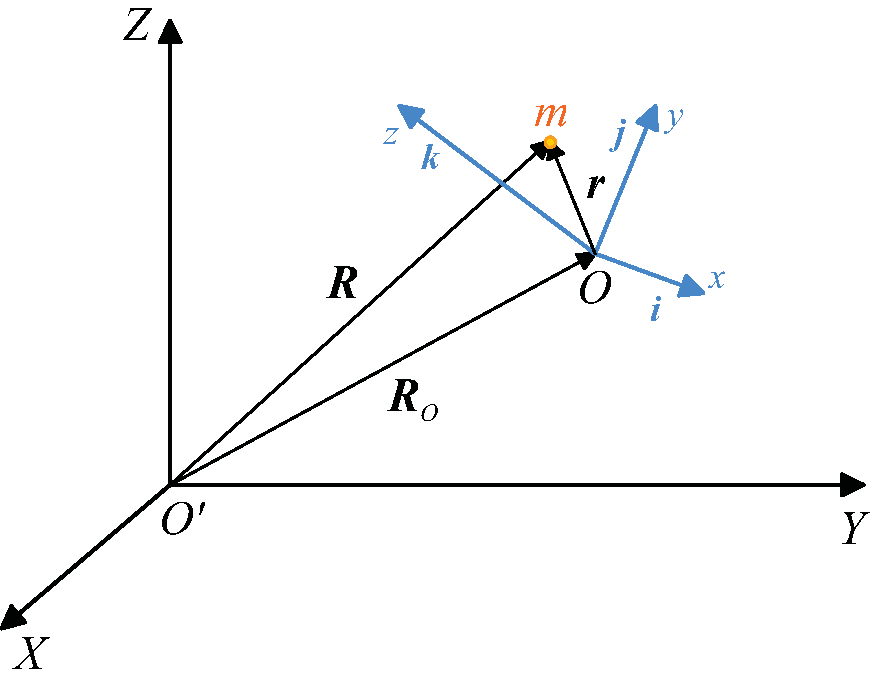
\includegraphics[width=0.4\linewidth]{pic/单质点角动量}
    \vspace*{-1em}
    \caption{质点$m$关于任意参考点$O$的角动量}
    \label{单质点角动量}
\end{figure}

在动坐标系中存在一个质量为$m$的质点,其\dy[线动量]{XDL}为
\begin{equation}
    \bm{p} = m \dot{\bm{R}}
    \nomenclature{$\bm{p}$}{质点的线动量 \nomrefpage}
\end{equation}
其中,$\bm{R}$为质点相对于惯性坐标系的位置向量(绝对位置向量)。

质点$m$的动量$\bm{p}$关于参考点$O$的\dy[角动量]{JDL}(或\dy[动量矩]{DLJ})定义为
\begin{equation}
    \bm{H}^O = \bm{r} \times m \dot{\bm{R}}
    \nomenclature{$\bm{H}^O$}{质点关于参考点$O$的角动量 \nomrefpage}
\end{equation}
其中,$\bm{r}$为质点$m$相对于参考点$O$的位置向量(相对位置向量)。由于$\bm{R} = \bm{R}_O + \bm{r}$,则有$\dot{\bm{R}} = \dot{\bm{R}}_O + \dot{r}$,那么
\begin{equation}
    \bm{H}^O = \bm{r} \times m \dot{\bm{r}} + \bm{r} \times m \dot{\bm{R}}_O
    \label{H1}
\end{equation}
其中,公式 \eqref{H1} 右侧第一项$\bm{r} \times m \dot{\bm{r}}$称为动坐标系$Oxyz$中的\dy[视角动量]{SJDL},用$\bm{H}^{\underline{O}}$表示;而另一项是因为点$O$运动引起的修正项。
\nomenclature{$\bm{H}^{\underline{O}}$}{质点的视角动量 \nomrefpage}

质点$P$关于参考点的角动量$\bm{H}^O$的时间导数(相对惯性系)为
\begin{align}
    \dot{\bm{H}}_O & = \dfrac{\d }{\d t} (\bm{r} \times m \dot{\bm{r}}) + m \dot{\bm{r}} \times \dot{\bm{R}}_O + m \bm{r} \times \ddot{\bm{R}}_O \notag                                                                                        \\[0.2em]
                   & = \underbrace{\,\,\, \dfrac{\d }{\d t} (\bm{r} \times m \dot{\bm{r}}) \,\,\,}_{{\footnotesize \mbox{视角动量的变化率}}}  - \underbrace{ \,\,\, \ddot{\bm{R}}_O \times m \bm{r} \,\,\,}_{\footnotesize  \makecell[c]{\quad \\[-1.54em] \mbox{点}\, O \,\mbox{加速度的影响项}}} - \underbrace{\,\,\, \dot{\bm{R}}_O \times m \dot{\bm{r}} \,\,\,}_{\footnotesize  \makecell[c]{\quad \\[-1.54em] \mbox{点}\, O \,\mbox{速度的影响项}}}
\end{align}

\sssection[单质点的动量矩定理]

角动量$\bm{H}^O$的变化率可以与关于$O$点的外力矩联系起来。作用在$m$上的力关于点$O$的力矩定义为
\begin{equation}
    \bm{T}^O = \bm{r} \times \bm{F}
\end{equation}
\nomenclature{$\bm{T}^O$}{关于点$O$的力矩 \nomrefpage}
由牛顿第二定律,有
\begin{equation}
    \bm{F} = m \ddot{\bm{R}}
\end{equation}
所以
\begin{equation}
    \bm{T}^O = \bm{r} \times m \ddot{R} = \bm{r} \times m (\ddot{\bm{R}}_O + \ddot{\bm{r}})
\end{equation}
由于$\dot{\bm{r}} \times \dot{\bm{r}} = 0$,所以
\begin{equation}
    \bm{T}^O = \dfrac{\d }{\d t} (\bm{r} \times m \dot{\bm{r}}) - \ddot{\bm{R}}_O \times m \bm{r}
\end{equation}
而$\dot{\bm{H}}_O  =  \dfrac{\d }{\d t} (\bm{r} \times m \dot{\bm{r}} ) - \ddot{\bm{R}}_O \times m \bm{r} - \ddot{\bm{R}}_O \times m \bm{r}$,对比可得

\theorem[单质点的动量矩定理]{
    \index{DZDDDLJDL@单质点的动量矩定理}
    \index{DLJDL@动量矩定理}
    对于单质点$m$相对于任意参考点$O$的角动量$\bm{H}^O$与作用在$m$上的力关于点$O$的力矩$\bm{T}^O$的关系为
    \begin{equation}
        \dot{\bm{H}}^O = \bm{T}^O - \dot{\bm{R}}_O \times m \dot{\bm{r}}
    \end{equation}
    特别地,如果参考点$O$是固定在惯性坐标系的一个点,那么$ \dot{\bm{R}}_O = 0$,即
    \begin{equation}
        \dot{\bm{H}}^O = \bm{T}^O
    \end{equation}
    这就表明,如果外加力矩为0,那么$\bm{H}^O$就是常量,即在外力矩为0的条件下,质点的\dy[角动量守恒]{JDLSH}。
}

\clearpage

\subsection{多质点系统的动量矩定理}
如图 \ref{多质点角动量} 所示,假设坐标系$O'XYZ$是一个惯性坐标系,$O$是其中的一个动参考点,以$O$为原点建立一个动坐标系$Oxyz$。
\begin{figure}[!htb]
    \centering
    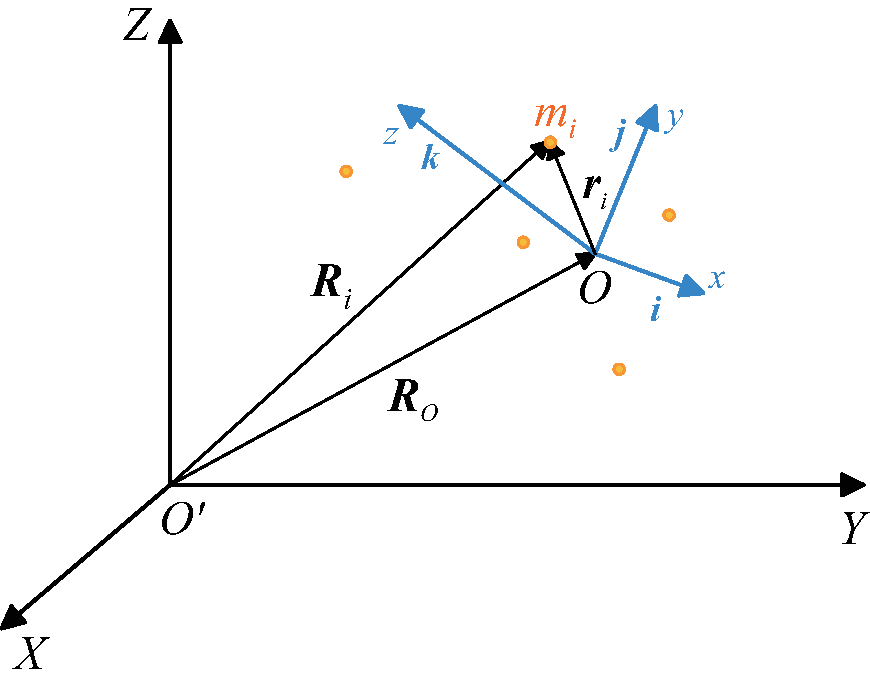
\includegraphics[width=0.4\linewidth]{pic/多质点角动量}
    \vspace*{-1em}
    \caption{某个质点$m_i$关于任意参考点$O$的角动量}
    \label{多质点角动量}
\end{figure}

在动坐标系中存在一个包含$N$个质点的多质点系统$A$,记第$i$个质点的质量为$m$,惯性系原点$O'$到这个质点的位置向量为$\bm{R}_i$,质点运动的绝对速度为$\bm{V}_i$。质点相对于动参考点的相对位置向量为$\bm{r}_i$,则有$\bm{R}_i = \bm{R}_O + \bm{r}_i$。

对于单个质点$m_i$其所受合外力为$\bm{F}_i$,那么其关于点$O$的力矩为$\bm{T}_i^O = \bm{r}_i \times \bm{F}_i$,那么整个质点系的外力关于$O$点的力矩为
\begin{equation}
    \bm{T}^O = \sum \bm{T}_i^O = \sum \bm{r}_i \times \bm{F}_i
\end{equation}

设多质点系统的总质量为$m = \displaystyle \sum m_i$,系统的总动量为$\bm{p} =  \displaystyle \sum m_i \bm{V}_i$,系统的质心为$C$,其绝对位置向量为$\bm{R}_C$,质心速度为$\bm{V}_C$,那么由单质点动量矩,单个质点$m_i$关于点$O$的动量矩为
\begin{equation*}
    \bm{H}_i^O = \bm{r}_i \times m_i \dot{r}_i - \bm{V}_O \times m_i \bm{r}_i
\end{equation*}
那么系统的动量矩为
\begin{equation}
    \bm{H}^O = \sum \bm{H}_i^O = \sum \bm{r}_i \times m_i \dot{\bm{r}}_i - \bm{V}_O \times \sum m_i \bm{r}_i
\end{equation}

\theorem[多质点系统的动量矩定理]
{
与单质点关于动参考点的动量矩定理类似,多质点系统关于动参考点$O$的动量矩定理为
\begin{align}
    \dot{\bm{H}}^O & = \sum \bm{T}_i^O - \bm{V}_O \times \sum m_i\dot{\bm{r}}_i \notag        \\
                   & = \bm{T}^O - \bm{V}_O \times \sum m_i (\bm{V}_O + \dot{\bm{r}}_i) \notag \\
                   & = \bm{T}^O - \bm{V}_O \times \sum m_i \bm{V}_i \notag                    \\
                   & = \bm{T}^O - \bm{V}^O \times \bm{p}
\end{align}
可以看出,多质点系统关于动参考系的动量矩的时间导数不仅和外力矩有关,还与动参考点的平移运动以及系统的线动量有关,即{\color{dy} 多质点系统的姿态运动和平移运动耦合}。\\
\hspace*{2em} 特别地,当参考点$O$取质心$C$时,由牛顿第二定律及冲量定理,有\\[-1.7em]
\begin{equation}
    \dot{\bm{p}} = \sum \bm{F}_i  = m \dot{\bm{V}}_C
    \vspace*{-0.4em}
\end{equation}
积分后得系统动量的表达式:$\bm{p} = m \bm{V}_C$。而由于动参考点$O$取$C$,有$\bm{V}_O \times \bm{p} = \bm{V}_C \times \bm{p} = \bm{V}_C \times (m \bm{V}_C) = 0$,那么\\[-1.5em]
\begin{equation}
    \dot{\bm{H}}_C = \bm{T}^C
    \label{多质点动量矩}
\end{equation}
}
\clearpage
\vspace*{-2.5em}

\summarize
[
\qquad 由多质点动量矩公式 \eqref{多质点动量矩} 可以看出,当系统质心$C$为参考点时,其动量矩定理具有和参考点取为固定点一样的简单形式,即{\color{dy}姿态运动和平移运动解耦}。这就是研究物体转动运动时常常取质心坐标系的原因。
]




\section{并矢}
为了更好理解并矢,我们先从简单的张量形式理解。
\subsection{张量}
实际上,\dy[张量]{ZL}是表示物理量的一种方式,具体而言就是用基向量表示一个物理量,张量的阶数$n$,表示物理量的基向量具有$n$个方向。常用的有:0阶张量,1阶张量,2阶张量。
\vspace*{1em}

\sssection[0阶张量]

\dy[0阶张量]{0JZL}为无基向量的张量,说明其只有值而没有方向,即\dy[标量]{BL},即
\begin{equation}
    A = \begin{cases}
        A
    \end{cases}
\end{equation}
在物理上,质量就是一个0阶张量,仅代表物体的质量,所以质点只能是一个点,因为它是0阶张量,没有方向。

\vspace*{1em}

\sssection[1阶张量]

\dy[1阶张量]{1JZL}为仅\textbf{1个方向的$3^1 = 3$个基向量}决定的张量,即三维\dy[向量]{XL},如图 \ref{一阶张量} 所示。任何一个1阶张量都可以用3个分量和3个基向量表示,即
\begin{equation}
    \bm{A} =
    \begin{cases}
        A_x & \bm{x} \\
        A_y & \bm{y} \\
        A_z & \bm{z}
    \end{cases}
\end{equation}
在物理上,一阶张量很常见,速度、加速度等都是一阶张量,具有大小的单个方向的物理量。

\begin{figure}[!htb]
    \centering
    \begin{minipage}{0.49\linewidth}
        \centering
        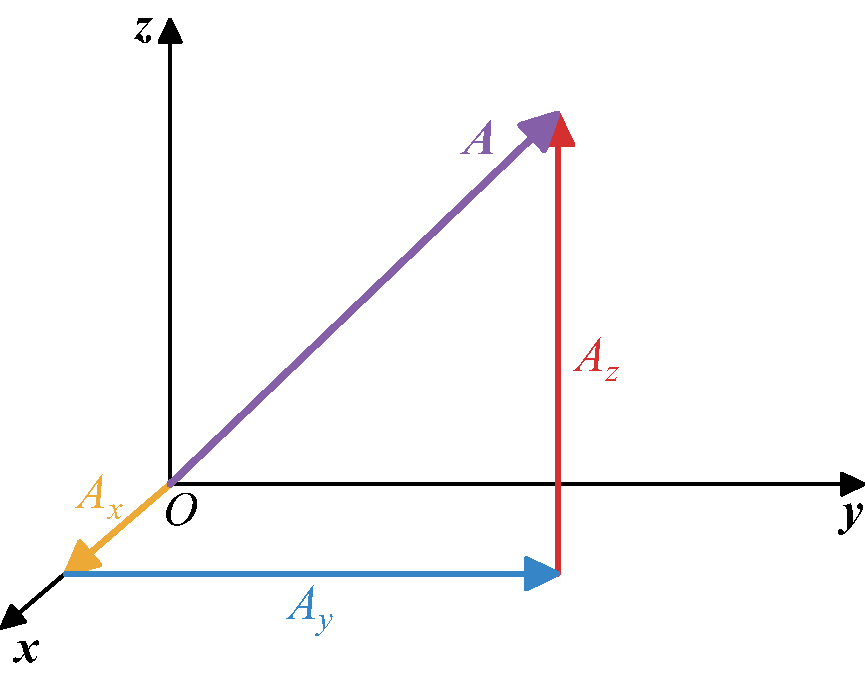
\includegraphics[width=0.92\linewidth]{pic/一阶张量}
        \captionof{figure}{1阶张量示意图}
        \label{一阶张量}
    \end{minipage}
    \begin{minipage}{0.49\linewidth}
        \centering
        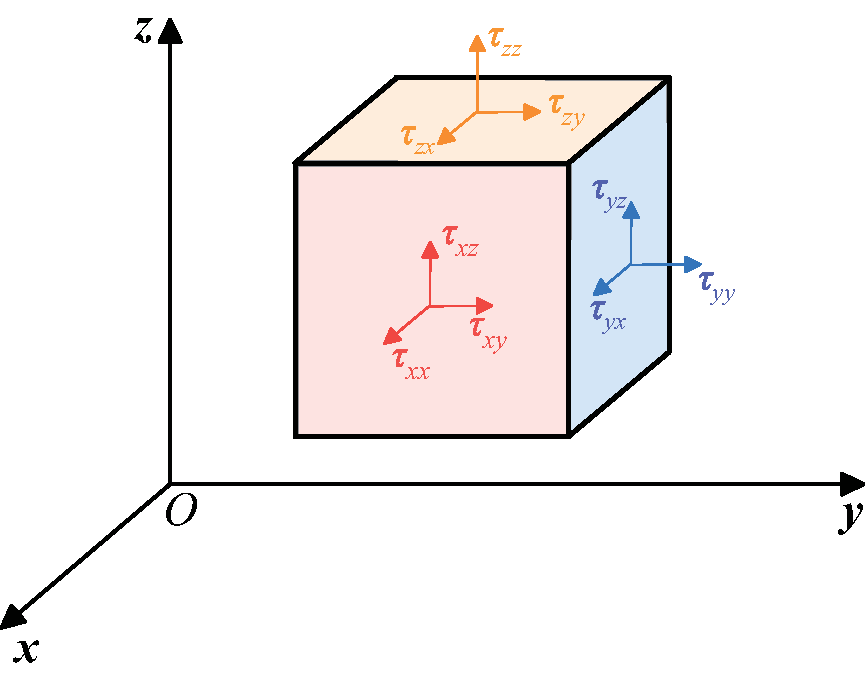
\includegraphics[width=0.92\linewidth]{pic/二阶张量}
        \captionof{figure}{2阶张量示意图}
        \label{二阶张量}
    \end{minipage}
\end{figure}
\newpage

\sssection[2阶张量]

\dy[2阶张量]{2JZL}为有\textbf{2个方向的$3^2 = 9$个基向量}决定的张量,如图 \ref{二阶张量} 所示。任何一个2阶张量都可以用9个分量和9个基向量表示,如表 \ref{2-9-1}, \ref{2-9-2} 所示。
\begin{table}[!htb]
    \begin{minipage}{0.5\linewidth}
        \centering
        \renewcommand\arraystretch{1.29}
        \setlength{\tabcolsep}{2.5em}{
            \begin{tabular}{|c|c|c|}
                \hline
                $A_{xx}$ & $A_{xy}$ & $A_{xz} $ \\
                \hline
                $A_{yx}$ & $A_{yy}$ & $A_{yz} $ \\
                \hline
                $A_{zx}$ & $A_{zy}$ & $A_{zz} $ \\
                \hline
            \end{tabular}
        }
        \caption{2阶张量的9个分量}
        \label{2-9-1}
        \renewcommand\arraystretch{1}
    \end{minipage}
    \begin{minipage}{0.5\linewidth}
        \centering
        \begin{tabular}{|c|c|c|}
            \hline
            \begin{minipage}{0.23\columnwidth}
                \centering
                \begin{tikzpicture}[>={Stealth[scale=1.2]}]
                    \path[draw,<-] (0,0) -- (0.8,0);
                    \path[draw,<-] (0,0.2) -- (0.8,0.2);
                \end{tikzpicture}
            \end{minipage}
             &
            \begin{minipage}{0.23\columnwidth}
                \centering
                \begin{tikzpicture}[>={Stealth[scale=1.2]}]
                    \path[draw,->] (0,0) -- (0.8,0);
                    \path[draw,<-] (0,0.2) -- (0.8,0.2);
                \end{tikzpicture}
            \end{minipage}
             &
            \begin{minipage}{0.23\columnwidth}
                \centering
                \begin{tikzpicture}[>={Stealth[scale=1.2]}]
                    \path[draw,<-] (0,0) -- (0.8,0);
                    \path[draw,->] (0.4,-0.35) -- (0.4,0.45);
                \end{tikzpicture}
            \end{minipage} \\
            \hline
            \begin{minipage}{0.23\columnwidth}
                \centering
                \begin{tikzpicture}[>={Stealth[scale=1.2]}]
                    \path[draw,<-] (0,0) -- (0.8,0);
                    \path[draw,->] (0,0.2) -- (0.8,0.2);
                \end{tikzpicture}
            \end{minipage}
             &
            \begin{minipage}{0.23\columnwidth}
                \centering
                \begin{tikzpicture}[>={Stealth[scale=1.2]}]
                    \path[draw,->] (0,0) -- (0.8,0);
                    \path[draw,->] (0,0.2) -- (0.8,0.2);
                \end{tikzpicture}
            \end{minipage}
             &
            \begin{minipage}{0.23\columnwidth}
                \centering
                \begin{tikzpicture}[>={Stealth[scale=1.2]}]
                    \path[draw,->] (0,0) -- (0.8,0);
                    \path[draw,->] (0.4,-0.35) -- (0.4,0.45);
                \end{tikzpicture}
            \end{minipage} \\
            \hline
            \begin{minipage}{0.23\columnwidth}
                \centering
                \begin{tikzpicture}[>={Stealth[scale=1.2]}]
                    \path[draw,<-] (0,0) -- (0.8,0);
                    \path[draw,->] (0.4,-0.35) -- (0.4,0.45);
                \end{tikzpicture}
            \end{minipage}
             &
            \begin{minipage}{0.23\columnwidth}
                \centering
                \begin{tikzpicture}[>={Stealth[scale=1.2]}]
                    \path[draw,->] (0,0) -- (0.8,0);
                    \path[draw,->] (0.4,-0.35) -- (0.4,0.45);
                \end{tikzpicture}
            \end{minipage}
             &
            \begin{minipage}{0.23\columnwidth}
                \centering
                \begin{tikzpicture}[>={Stealth[scale=1.2]}]
                    \path[draw,->] (0,-0.4) -- (0,0.4);
                    \path[draw,->] (0.2,-0.4) -- (0.2,0.4);
                \end{tikzpicture}
            \end{minipage} \\
            \hline
        \end{tabular}
        \caption{2阶张量9个基向量的方向}
        \label{2-9-2}
    \end{minipage}
\end{table}

在物理上,材料力学的\dy[应力张量]{YLZL}就是一个2阶张量。如图 \ref{二阶张量} 所示,在$x$轴为法向的面上收到三个力:沿着$x$轴方向的力,沿着$y$轴方向的力和沿着$z$轴方向的力,其他两个方向的面同理。也就是说,应力张量$\bm{\tau}$表示的是不同方向($\bm{x}, \bm{y}, \bm{z}$)的面受到3个不同方向的力$\bm{\tau}_x, \bm{\tau}_y, \bm{\tau}_z$,因此其基向量具有两个方向,一个表示受力面的方向,另一个表示受力面所受力的方向,即
\begin{equation}
    \bm{\tau} =
    \begin{bmatrix}
        \tau_{xx} & \tau_{xy} & \tau_{xz} \\
        \tau_{yx} & \tau_{yy} & \tau_{yz} \\
        \tau_{zx} & \tau_{zy} & \tau_{zz}
    \end{bmatrix}
\end{equation}
同样地,在理论力学中,\dy[惯性张量]{GXZL}也是一个2阶张量,即
\begin{equation}
    \bm{I} =
    \begin{bmatrix}
        I_{xx} & I_{xy} & I_{xz} \\
        I_{yx} & I_{yy} & I_{yz} \\
        I_{zx} & I_{zy} & I_{zz}
    \end{bmatrix}
\end{equation}

\subsection{并矢的定义}
在介绍了张量的定义和张量的分类后,我们可以由此引入并矢的定义。

\defination[并矢]
{
    \dy[并矢]{BS}是向量运算,表示为一系列双矢量的不定乘积之和,是物理对象的固有属性,也称为\textbf{2阶张量}。其既不是点乘也不是叉乘,可以理解为单纯地把两个向量并置而不做任何运算,即
    \begin{equation}
        \mathbb{Z} = \bm{a} \bm{b}
        \nomenclature{$\mathbb{Z}$}{并矢 \nomrefpage}
    \end{equation}
    由于并矢的特性,它只是单纯地把两个向量并置而不做任何运算,因此,其在基向量$\ubm{e}$中有9个基向量(因为$\bm{i}\bm{i}$不作任何运算,可以理解为新的基向量,所以一共有$3^2 = 9$个基向量),即
    \begin{equation}
        \mathbb{Z} = \bm{a} \bm{b} = \sum_{i=1}^{3}\sum_{j=1}^{3} a_ib_j \bm{e}_i \bm{e}_j =  \sum_{i=1}^{3}\sum_{j=1}^{3} Z_{ij} \bm{e}_i \bm{e}_j
    \end{equation}
    其中,$Z_{ij}$称为并矢$\mathbb{Z}$在$\ubm{e}$中的坐标或分量,即
    \begin{equation}
        \ubm{Z} =
        \begin{bmatrix}
            Z_{11} & Z_{12} & Z_{13} \\
            Z_{21} & Z_{22} & Z_{23} \\
            Z_{31} & Z_{32} & Z_{33}
        \end{bmatrix}
        =
        \begin{bmatrix}
            a_1b_1  & a_1b_2  & a_1 b_3 \\
            a_2 b_1 & a_2b_2  & a_2b_3  \\
            a_3b_1  & a_3 b_2 & a_3b_3
        \end{bmatrix}
        = \ubm{a}\cdot\ubm{b}^\T
        \qquad \Rightarrow \qquad
        \mathbb{Z} = \ubm{e}^\T \ubm{Z} \ubm{e}
    \end{equation}
}

\newpage
若并矢坐标矩阵$\ubm{Z}$为单位矩阵$\ubm{E}_3$,那么这个并矢称为\dy[单位并矢]{DWBS}
\begin{equation}
    \mathbb{E} = \ubm{e}^\T \ubm{e} 
    = \bm{e}_1 \bm{e}_1 + \bm{e}_2\bm{e}_2 + \bm{e}_3\bm{e}_3
    \nomenclature{$\mathbb{E}$}{单位并矢 \nomnorefpage}
\end{equation}

若将并矢$\mathbb{Z}$中的两个向量$\bm{a}\bm{b}$交换顺序,可以得到\dy[共轭并矢]{GEBS}
\begin{equation}
    \mathbb{Z}^* = \bm{b}\bm{a}
    \nomenclature{$\mathbb{Z}^*$}{并矢$\mathbb{Z}$的共轭并矢 \nomrefpage}    
\end{equation}
其中,相互共轭的并矢,它们的坐标矩阵是相互转置的:
\begin{equation}
    \ubm{D}^* = \ubm{D}^\T
\end{equation}


\subsection{并矢的运算法则}
\sssection[并矢的线性运算]

两个并矢的和与差的结果为并矢,即
\begin{equation}
    \mathbb{Z} = \mathbb{D} \pm \mathbb{G}    
\end{equation}
\vspace*{0.1em}

\sssection[并矢与向量点乘]

并矢与向量点乘得到的是一个向量,即
\begin{equation}
    \bm{u} = \mathbb{Z} \cdot \bm{v} = \bm{a}\left(\bm{b} \cdot \bm{v}\right) = \ubm{e}^\T \ubm{Z} \ubm{e} \ubm{e}^\T \ubm{v} = \ubm{e}^\T \ubm{Z} \ubm{v}
\end{equation}
\vspace*{0.1em}

\sssection[并矢与向量叉乘]

并矢与向量叉乘得到的是一个并矢,即
\begin{align}
    \mathbb{C} &= \mathbb{Z} \times \bm{v} = \bm{a}(\bm{b} \times \bm{v}) \\
    \mathbb{C} &= \bm{v} \times \mathbb{Z} = (\bm{v} \times \bm{a})\bm{b} 
\end{align}
并矢与向量叉乘不满足交换律,但满足分配律。
\vspace*{1em}

\sssection[并矢的并矢的点乘]

两个并矢点乘得到的是一个并矢,记$\mathbb{D} = \bm{a}\bm{b}, \, \mathbb{G} = \bm{c}\bm{d}$,那么
\begin{equation}
    \mathbb{C} = \mathbb{D} \cdot \mathbb{G} = \bm{a} (\bm{b} \cdot \bm{c}) \bm{d} = (\bm{b} \cdot \bm{c})\bm{a}\bm{d}
\end{equation}
并矢之间的点乘不满足交换律。
\vspace*{1em}


\subsection{向量双重叉乘与并矢}
由向量叉乘公式,
\begin{equation}
    \bm{a} \times (\bm{b} \times \bm{c}) = \bm{b}(\bm{a}\cdot\bm{c}) - \bm{a}(\bm{b} \cdot \bm{c})
\end{equation}
由并矢的定义及并矢与向量的点乘的定义,那么
\begin{equation}
    \bm{b}(\bm{a} \cdot \bm{c}) - \bm{a}(\bm{b} \cdot \bm{c}) = (\bm{b}\bm{a} - \bm{a}\bm{b})\cdot \bm{c}
\end{equation}

可以将$\bm{b}\bm{a} - \bm{a}\bm{b}$在向量基$\ubm{e}$下分解,可以得到
\begin{equation*}
    \bm{b}\bm{a} - \bm{a}\bm{b} = \ubm{e}^\T (\ubm{b}\ubm{a}^\T - \ubm{a}\ubm{b}^\T)\ubm{e}
\end{equation*}






















